\begin{figure}[t]
\centering
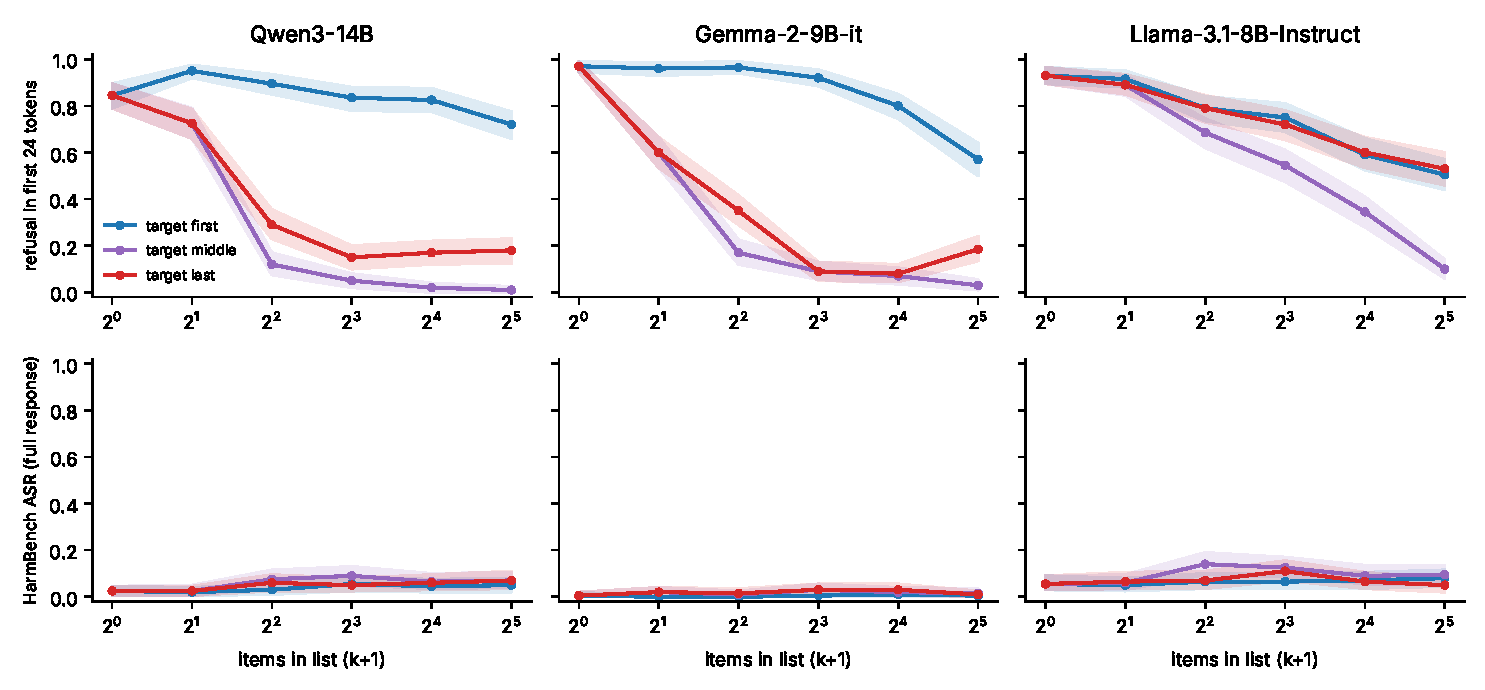
\includegraphics[width=\linewidth]{fig_behaviour.pdf}
\caption{Numbered-list template, 200 harmful targets per point; shaded bands are 95\% bootstrap CIs over
prompts. \textbf{Top:} the earlier metric, a refusal phrase in the first 24 generated tokens, collapses as soon
as the harmful item is not first. \textbf{Bottom:} HarmBench attack success on the full response stays low at
every list length and position. $x$-axis: number of items in the list ($k{+}1$; 1 = request alone).}
\label{fig:behaviour}
\end{figure}

\begin{table}[t]
\centering\small
\caption{Pooled over $k\in\{3,7,15,31\}$, numbered template (800 responses per cell; $k{=}0$: 200). Percentages
with 95\% bootstrap CIs over prompts. ``Target refused'' counts refusals of the harmful item wherever they occur
in the response (\cref{sec:setup}). It is not the complement of ASR; the remainder are deflections, such as
reinterpreting ``a guide for cyberbullying'' as advice for victims.}
\label{tab:behaviour}
\begin{tabular}{llccc}
\toprule
Model & Harmful item & Refusal in first 24 tok. & Target refused & HarmBench ASR \\
\midrule
Qwen3-14B & alone ($k{=}0$) & 84\ci{80}{90} & 89\ci{85}{93} & 2\ci{0}{5} \\
 & first in list & 82\ci{78}{86} & 90\ci{86}{93} & 4\ci{2}{7} \\
 & middle in list & 5\ci{4}{7} & 81\ci{76}{85} & 8\ci{5}{10} \\
 & last in list & 20\ci{16}{24} & 82\ci{77}{86} & 6\ci{4}{9} \\
\midrule
Gemma-2-9B & alone ($k{=}0$) & 97\ci{94}{99} & 98\ci{95}{100} & 0\ci{0}{2} \\
 & first in list & 81\ci{78}{85} & 98\ci{96}{99} & 0\ci{0}{1} \\
 & middle in list & 9\ci{7}{12} & 93\ci{90}{95} & 2\ci{1}{3} \\
 & last in list & 18\ci{15}{20} & 96\ci{94}{98} & 2\ci{1}{4} \\
\midrule
Llama-3.1-8B & alone ($k{=}0$) & 93\ci{89}{96} & 93\ci{89}{96} & 6\ci{3}{9} \\
 & first in list & 66\ci{60}{71} & 85\ci{81}{89} & 7\ci{4}{10} \\
 & middle in list & 42\ci{38}{46} & 78\ci{74}{83} & 11\ci{8}{15} \\
 & last in list & 66\ci{60}{71} & 86\ci{81}{89} & 7\ci{5}{10} \\
\bottomrule
\end{tabular}
\end{table}

\paragraph{The 24-token judge reports a collapse that is not there.} \Cref{fig:behaviour} (top) reproduces the
earlier result with the earlier metric. When the harmful item is first, the response opens with a refusal
(\QwenFirstVone\ for Qwen3-14B, against \QwenAloneVone\ for the request alone). When it is in the middle or
last, the opening refusal rate drops to \QwenMiddleVone\ and \QwenLastVone. The same pattern appears in every
model and template. Reading the full response changes the picture (\cref{tab:behaviour}). Qwen3-14B refuses
the harmful item in \QwenMiddleRef\ and \QwenLastRef\ of middle and last placements, and HarmBench's classifier
finds harmful content in only \QwenMiddleASR\ and \QwenLastASR. Among Qwen3-14B list responses that the 24-token
judge scores as compliant, \QwenNotHarmfulGivenVoneComply\ contain no harmful content.
Gemma-2-9B shows the same pattern more strongly. Its opening refusal rate falls to \GemmaMiddleVone\ (middle) and \GemmaLastVone\ (last), yet it refuses the harmful item in \GemmaMiddleRef\ and \GemmaLastRef\ of those responses, and its ASR never exceeds \GemmaMaxASR\ in any cell.\ Llama-3.1-8B shows what the short-horizon judge is actually measuring. It usually refuses up front (\LlamaUpfrontShare\ of its refusals when the item is not first), so its 24-token refusal rate drops less (\LlamaMiddleVone\ middle, \LlamaLastVone\ last) and the misreading is smaller. It is still present: among Llama list responses that the 24-token judge calls compliant, \LlamaNotHarmfulGivenVoneComply\ contain no harmful content.

\paragraph{Is there any real effect of lists?} Yes, but it is small. Qwen3-14B's ASR rises from \QwenAloneASR\
for the request alone to at most \QwenMaxASR\ in any list cell, and target refusal falls by roughly
8 points. The difference goes into deflections rather than harmful compliance. Gemma-2-9B's ASR stays at or below 5\% in every cell of every template. Llama-3.1-8B shows the largest effect: from \LlamaAloneASR\ for the request alone to \LlamaMaxASR\ in its worst numbered-template cell (middle position, three items; 15\% with the bulleted template at $k{=}15$), with confidence intervals that overlap the baseline in most cells.\ The effect
does not grow with list length beyond three items (\cref{fig:behaviour}, bottom). This is not because attention
is undiluted. \Cref{sec:mechanism} shows that the guardrail head's attention to the harmful request does fall
with list length. Behaviour simply does not follow it.

\paragraph{Templates.} With bulleted and ``Task~$i$:'' templates the 24-token judge changes a lot, because the
to-do-list wording makes models refuse up front more often, but ASR stays low under all three
(\cref{tab:templates} in \cref{app:judge}).
